\title{Icecast2}

\chapter{Introduction}
%{{{

\section{What is Icecast?}
%{{{

\begin{itemize}
\item Icecast is a streaming media server which currently supports Ogg
Vorbis/Theora, Opus, WebM and MPEG Audio Layer 3 (MP3) streams.
\end{itemize}

%}}}

\section{Licensing}
%{{{

\begin{itemize}
\item Icecast is distributed under the
  \href{http://www.gnu.org/licenses/gpl.html}{GNU GPL, version 2},
  which basically means:
\begin{enumerate}
\item You can use the source code to develop new open source GNU GPL
  V2 applications and
\item you can NOT use the source code to develop propietary applications.
\end{enumerate}
\end{itemize}

%}}}

%}}}

\chapter{Architecture}
%{{{

\begin{itemize}
\item \textbf{Source Clients:} Send the content to Icecast servers.
\item \textbf{Servers:} Sends content to Listeners and Relay Servers.
\item \textbf{Listeners:} Plays the content.
\item \textbf{Relay servers:} Act as listeners to servers, but are Servers.
\end{itemize}
\fig{600}{icecast-arq}

%}}}

\chapter{Setup}
%\chapter{Essential Server and Relay Server setup}
%{{{

\section{The configuration file}
%{{{

\begin{itemize}
\item Edit the \texttt{/etc/icecast2/icecast.xml} file and set:
\begin{enumerate}
\item The \texttt{<source-password>}, which will be used for the
  source client authentication,
\item \texttt{<admin-password>} that will be used for authenticating
  admin features of icecast.
\end{enumerate}
\item By default, Icecast2 sends data to listeners throught the port 8000.
\end{itemize}

%}}}

\section{Testing possible /etc/icecast2/icecast.xml syntax problems}
%{{{

\lstset{language=bash,
  basicstyle=\normalsize\ttfamily,
  %numbers=left,
  %frame=shadowbox,
  % numberstyle=\tiny, 
  keywordstyle=\color{blue}\textbf,
  % tabsize=4,
  % numbersep=15pt,
  % stepnumber=1,
  commentstyle=\color[rgb]{0.133,0.545,0.133},
  stringstyle=\color[rgb]{0.627,0.126,0.941},
  % upquote=true,
  % aboveskip={2\baselineskip},
  % columns=fixed,
  % showstringspaces=false,
  % extendedchars=true,
  breaklines=true,
  prebreak=\raisebox{0ex}[0ex][0ex]{\ensuremath{\hookleftarrow}}
}
\begin{lstlisting}
  sudo xmllint /etc/icecast2/icecast.xml
\end{lstlisting}
\begin{itemize}
\item If you get only the content of
  \texttt{/etc/icecast2/icecast.xml}, the file is OK.
\end{itemize}

%}}}

%}}}

%\chapter{Extra Server and Relay Server setup}
%{{{

\section{Limits}
%{{{

\lstset{language=xml,
  basicstyle=\normalsize\ttfamily,
  %numbers=left,
  %frame=shadowbox,
  % numberstyle=\tiny, 
  keywordstyle=\color{blue}\textbf,
  % tabsize=4,
  % numbersep=15pt,
  % stepnumber=1,
  commentstyle=\color[rgb]{0.133,0.545,0.133},
  stringstyle=\color[rgb]{0.627,0.126,0.941},
  % upquote=true,
  % aboveskip={2\baselineskip},
  % columns=fixed,
  % showstringspaces=false,
  % extendedchars=true,
  breaklines=true,
  prebreak=\raisebox{0ex}[0ex][0ex]{\ensuremath{\hookleftarrow}}
}

\begin{lstlisting}
<limits>

    <!----------------------------------------------------------------->
    <!-- Total number of concurrent clients supported by the server. -->
    <clients>100</clients>                                       <!---->
    <!----------------------------------------------------------------->

    <!-- Maximum number of connected sources supported by the server. -->
    <sources>2</sources>

    <!-- the number of threads that are started to handle client
    connections. -->
    <threadpool>5</threadpool>

    <!-- This is the maximum size (in bytes) of the stream queue (for
    a channel) which uncouples the source client and the
    listeners. -->
    <queue-size>524288</queue-size>

    <!-- Unused. -->
    <client-timeout>30</client-timeout>
    
    <!-- The maximum time (in seconds) to wait for a request to come
    in once the client has made a connection to the server. -->
    <header-timeout>15</header-timeout>

    <!-- If a connected source does not send any data within this
    timeout period (in seconds), then the source connection will be
    removed from the server. -->
    <source-timeout>10</source-timeout>

    <!-- Deprecated. Use burst-size instead. -->
    <burst-on-connect>1</burst-on-connect>

    <!-- the amount of data (in bytes) to burst to a client at
    connection time. -->
    <burst-size>65535</burst-size>

</limits>
\end{lstlisting}

%}}}

\section{Authentication}
%{{{

\begin{lstlisting}
<authentication>

    <!------------------------------------------------------------------------>
    <!-- The unencrypted password used by sources to connect to the server. -->
    <source-password>hackme</source-password>                           <!---->
    <!------------------------------------------------------------------------>

    <!------------------------------------------------------------------------------>
    <!-- The unencrypted password used by relay servers to connect to the server. -->
    <relay-user>relay</relay-user>                                            <!---->
    <relay-password>hackme</relay-password>                                   <!---->
    <!------------------------------------------------------------------------------>
  
    <!---------------------------------------------------------------->
    <!-- The unencrypted password used for administration purposes. -->
    <admin-user>admin</admin-user>                              <!---->
    <admin-password>hackme</admin-password>                     <!---->
    <!---------------------------------------------------------------->

</authentication>
\end{lstlisting}

%}}}

\section{\href{http://dir.xiph.org}{Stream Directory} Settings (disabled by default)}
%{{{

\begin{lstlisting}
<directory>

    <!-- The maximum time the server will wait for a response from a
    particular directory server. -->
    <yp-url-timeout>15</yp-url-timeout>

    <!-- URL of the directory server -->
    <yp-url>http://dir.xiph.org/cgi-bin/yp-cgi</yp-url>

</directory>
\end{lstlisting}

%}}}

\section{Listening settings}
%{{{

%{{{

\begin{lstlisting}
<!-- You may have multiple <listen-socket> elements -->
<listen-socket>

     <!------------------------------------------------------------------>
     <!-- The TCP port that will be used to accept client connections. -->
     <port>8000</port>                                             <!---->
     <!------------------------------------------------------------------>

     <!-- An optional IP address that can be used to bind to a
          specific network card. If not supplied, then it will bind to all
          interfaces. -->
     <!-- <bind-address>127.0.0.1</bind-address> -->

</listen-socket>
\end{lstlisting}

%}}}

\subsection{Shoutcast compatibility}
%{{{

\begin{lstlisting}
<!-- Shoutcast clients does not specifies mount points.  -->
<shoutcast-mount>/live.nsv</shoutcast-mount>

<listen-socket>
     <port>8000</port>
</listen-socket>

<listen-socket>
     <!-- You need an extra port to communicate with Shoutcast clients. -->
     <port>8001</port>
     <shoutcast-compat>1</shoutcast-compat>
</listen-socket>
\end{lstlisting}

%}}}

%}}}

\section{Relaying Streams}
%{{{

%{{{

\subsection{Master Relay}
\begin{lstlisting}
<!-- Master server relay is only supported between icecast2 servers. -->

<!-- IP of the server which contains the mountpoints to be relayed
     (master server) -->
<!-- <master-server>127.0.0.1</master-server> -->

<!-- TCP port where the master server is listening. -->
<!-- <master-server-port>8001</master-server-port> -->

<!-- Interval (in seconds) that the relay server (this server) will
     poll the master server for any new mountpoints to relay. -->
<!-- <master-update-interval>120</master-update-interval> -->

<!-- Relay username and password on the master server. -->
<!-- <master-username>relay</master-username> -->
<!-- <master-password>hackme</master-password> -->

<!-- Only relay if there is at least one listener. -->
<!-- <relays-on-demand>0</relays-on-demand> -->
\end{lstlisting}

%}}}

\subsection{Specific Mountpoint Relay}
%{{{

\begin{lstlisting}
<!--
<relay>
     <!-- Server to be relayed. -->
     <server>127.0.0.1</server>
     <port>8001</port>

     <!-- Mountpoint to be relayed. -->
     <mount>/example.ogg</mount>

     <!-- Local mountpoint name. -->
     <local-mount>/different.ogg</local-mount>

     <!-- The source of the relay may require authentication itself. -->
     <username>joe</username>
     <password>soap</password>

     <!-- If you are relaying a Shoutcast stream, you may want to
          specify this indicator to also relay the metadata (song titles)
          that are part of the Shoutcast data stream (1=enabled,
          0=disabled). -->
     <relay-shoutcast-metadata>0</relay-shoutcast-metadata>

     <!-- Will only retrieve is there are listeners. -->
     <on-demand>1</on-demand>
</relay>
-->
\end{lstlisting}

%}}}

%}}}

\section{Mount Specific Settings}
%{{{
\begin{lstlisting}

<!-- The purpose of the mount definition is to state certain
      information that can override either global/default settings or
      settings provided from the incoming stream.

<mount>
     <!-- The name of the mount point for which these settings apply. -->
     <mount-name>/example-complex.ogg</mount-name>

     <!-- Username and password that a source must use to connect
          using this mountpoint. -->
     <username>othersource</username>
     <password>hackmemore</password>

     <!-- Maximum number of listeners that can be attached to this
          mountpoint. -->
     <max-listeners>1</max-listeners>

     <!-- Time a listener will stay connected. -->
     <max-listener-duration>3600</max-listener-duration>

     <!-- The filename which will be a dump of the stream coming
          through on this mountpoint. -->
     <dump-file>/tmp/dump-example1.ogg</dump-file>

     <!-- File those contents will be sent to new listeners when they
          connect but before the normal stream is sent. -->
     <intro>/intro.ogg</intro>

     <!-- Mountpoint that clients are automatically moved to if the
          source shuts down or is not streaming at the time a listener
          connects. -->
     <fallback-mount>/example2.ogg</fallback-mount>

     <!-- Enable/disable fallback. -->
     <fallback-override>1</fallback-override>

     <!-- When the max listener count for the mountpoint has been
          reached new listerners will fallback (or not). -->
     <fallback-when-full>1</fallback-when-full>

     <!-- Charset used for metadata. -->
     <charset>ISO8859-1</charset>

     <!-- -1: The source client/relay determines if the mountpoint
              should advertise. 0: no advertising and 1: force to
              advertise. -->
     <public>1</public>

     <!-- New stream name. -->
     <stream-name>My audio stream</stream-name>

     <!-- New stream description. -->
     <stream-description>My audio description</stream-description>

     <!-- New stream URL. -->
     <stream-url>http://some.place.com</stream-url>

     <!-- New stream genre. -->
     <genre>classical</genre>

     <!-- New stream info bit-rate. -->
     <bitrate>64</bitrate>

     <!-- New stream type. -->
     <type>application/ogg</type>

     <!-- New stream subtype. -->
     <subtype>vorbis</subtype>

     <!-- To prevent this mount from being shown on the xsl pages. -->
     <hidden>1</hidden>

     <!-- Burst size which overrides the default burst size as defined
          in limits. The value is in bytes. -->
     <burst-size>65536</burst-size>

     <!-- This optional setting specifies what interval, in bytes,
          there is between metadata updates within shoutcast compatible
          streams. -->
     <mp3-metadata-interval>4096</mp3-metadata-interval>

     <!- -This specifies that the named mount point will require
          listener (or source) authentication. -->
     <authentication type="xxxxxx">
     </authentication>

     <!-- State a program that is run when the source is started. -->
     <on-connect>/home/icecast/bin/source-start</on-connect>

     <!-- State a program that is run when the source ends. -->
     <on-disconnect>/home/icecast/bin/source-end</on-disconnect>
</mount>
-->
\end{lstlisting}

%}}}

\section{Security settings}
%{{{

\begin{lstlisting}
<security>

    <!-- Specifies whether a chroot() will be done when the server is
         started. -->
    <chroot>0</chroot>

    <!-- User and group that will own the icecast process when it is
         started. -->
    <changeowner>
        <user>nobody</user>
        <group>nogroup</group>
    </changeowner>
</security>
\end{lstlisting}

%}}}

\section{Path settings}
%{{{

\begin{lstlisting}
<paths>

    <!-- Base directory that is chrooted to when the server is started. -->
    <basedir>./</basedir>

    <!-- Base directory used for logging. --> 
    <logdir>./logs</logdir>

    <!-- File to write at startup and to remove at normal shutdown. -->
    <pidfile>./icecast.pid</pidfile>

    <!-- Base directory used for all static file requests. For
         example, if webroot is set to /var/share/icecast2, and a request
         for http://server:port/mp3/stuff.mp3 comes in, then the file
         /var/share/icecast2/mp3/stuff.mp3 will be served. -->
    <webroot>./web</webroot>

    <!-- Hold the XSLT scripts used for the web-based admin interface. -->
    <adminroot>./admin</adminroot>

    <!-- File that contains a list of IP addresses that will be
         allowed to connect to icecast. -->
    <allow-ip>/path/to/ip_allowlist</allow-ip>

    <!-- File that contains a list of IP addressess that will be
         dropped immediately. -->
    <deny-ip>/path_to_ip_denylist</deny-ip>

    <!-- Aliases are used to provide a way to create multiple
         mountpoints that refer to the same mountpoint. -->
    <alias source="/foo" dest="/bar"/> </paths>
\end{lstlisting}

%}}}

\section{Logging settings}
%{{{

\begin{lstlisting}
<logging>

    <!-- Into this file, all requests made to the icecast2 will be
         logged. -->
    <accesslog>access.log</accesslog>

    <!-- All icecast generated log messages will be written to this
         file. -->
    <errorlog>error.log</errorlog>

    <!-- Into this file, a log of all metadata for each mountpoint
         will be written. -->
    <playlistlog>playlist.log</playlistlog>

    <!-- If this value is set, then icecast will append a timestamp to
         the end of the logfile name when logsize has been reached. If
         disabled, then the default behavior is to rename the logfile to
         logfile.old (overwriting any previously saved logfiles). We
         disable this by default to prevent the filling up of filesystems
         for people who don't care (or know) that their logs are
         growing. -->
    <!-- <logarchive>1</logarchive> -->

    <!-- Indicates what messages are logged by icecast. 4 Debug, 3
         Info, 2 Warn, 1 Error. -->
    <loglevel>4</loglevel>
</logging>
\end{lstlisting}

%}}}

\section{Miscelaneous settings}
%{{{

\begin{lstlisting}
<!-- The hostname other people will use to connect to your server. -->
<hostname>localhost</hostname>

<!-- The location of the server. */
<location>earth</location>

<!-- Contact details for getting in touch with the server
     administrator. -->
<admin>icemaster@localhost</admin>

<!-- If ``1'', all files are served relative to the path specified in
     the <paths><webroot> configuration setting. -->
<fileserve>1</fileserve>

<!-- To override the default server identification. -->
<server-id>icecast 2.3</server-id>
\end{lstlisting}

%}}}

%}}}

\chapter{Usage}

\section{Installation}
\begin{verbatim}
# Debians:
sudo apt-get install icecast2 # Configure it!

# The server is running now and scheduled to run after rebotting the host.
# However, if this does not work, it can be launched manually with:
sudo icecast2 -c /etc/icecast2/icecast.xml

# Or even better with:
sudo /etc/init.d/icecast2 restart
\end{verbatim}

\lstset{language=bash,
  basicstyle=\normalsize\ttfamily,
  %numbers=left,
  %frame=shadowbox,
  % numberstyle=\tiny, 
  keywordstyle=\color{blue}\textbf,
  % tabsize=4,
  % numbersep=15pt,
  % stepnumber=1,
  commentstyle=\color[rgb]{0.133,0.545,0.133},
  stringstyle=\color[rgb]{0.627,0.126,0.941},
  % upquote=true,
  % aboveskip={2\baselineskip},
  % columns=fixed,
  % showstringspaces=false,
  % extendedchars=true,
  breaklines=true,
  prebreak=\raisebox{0ex}[0ex][0ex]{\ensuremath{\hookleftarrow}}
}

\section{Checking the server status}
%{{{

\begin{itemize}
\item Options:
  \begin{enumerate}
  \item Check the error.log file for the 'server started' message. It
    should include something like:
\begin{verbatim}
head /var/log/icecast2/error.log
#[2003-10-31  13:04:49] INFO main/main.c Icecast 2.3.0 server started
\end{verbatim}
  \item By visiting the main page:
\begin{verbatim}
firefox http://serverIP:port/admin/stats.xml &
\end{verbatim}
  \item Telneting the \texttt{serverIP:port}.
\begin{verbatim}
telnet localhost 8000
\end{verbatim}
  \end{enumerate}
\end{itemize}

%}}}

\section{Configuring a Source Client}
%{{{

\begin{itemize}
\item A Source Client provides content to a Server or Relay Server.
\item It is neccesary to:
  \begin{enumerate}
  \item Specify the IP address and the port of the icecast server.
  \item Choose a mountpoint. Example:
\begin{verbatim}
# oggfwd server_host server_port source_pass mountpoint < file.ogg
oggfwd localhost 8000 hackme /ejemplo.ogg < Big_Buck_Bunny_small.ogv
\end{verbatim}
  \end{enumerate}
\item Verify that it is connected by retrieving the stats.xml file
  from Icecast.
\end{itemize}

%}}}

\section{Configuring a Listener}
%{{{

\begin{itemize}
\item A Listener usually plays the content. 
\item It is necessary to specify a \texttt{.m3u} or directly the
  mountpoint. Examples:
\begin{verbatim}
vlc http://localhost:8000/mystream.ogg.m3u
vlc http://localhost:8000/mystream.ogg
wget http://localhost:8000/mystream.ogg
firefox http://localhost:8000/mystream.ogg
\end{verbatim}

\end{itemize}

%}}}

\section{The administration interface}
%{{{

\begin{itemize}
\item Available at (example):
\begin{verbatim}
http://localhost:8000/admin/stats.xsl
\end{verbatim}
\item Functionality:
\begin{enumerate}
\item Gather statistics,
\item move listeners from mountpoint to mountpoint,
\item disconnect connected sources,
\item disconnect connected listeners,
\item
  \href{http://www.icecast.org/docs/icecast-trunk/icecast2_admin.html}{and
    more ...}.
\end{enumerate}
\end{itemize}

%}}}

\section{Feeding Icecast}
\lstset{language=bash}
\begin{lstlisting}
# Capturing the WebCam and sending the stream by using ffmpeg + ffmpeg2theora + oggfwd:
ffmpeg -f alsa -i default \
  -f video4linux2 -s 640x480 -r 30 -i /dev/video0 -f avi - | \
ffmpeg2theora -a 0 -v 5 -f avi -x 640 -y 480 -o /dev/stdout - | \
oggfwd localhost 8000 hackme /ejemplo.ogg

# Capturing the WebCam and sending the stream with VLC:
cvlc v4l2:///dev/video0 :input-slave=alsa:// \
  --sout '#transcode{vcodec=theo,vb=800,width=640,\
heigh=480,acodec=vorb,ab=64,channels=2,samplerate=44100}:\
duplicate{dst=std{access=shout,mux=ogg,dst=source:\
hackme@localhost:8000/ejemplo.ogg},dst=display}' :sout-keep
\end{lstlisting}

\section{Capturing a Icecast's stream}
\label{sec:captura_stream_icecast}
\begin{verbatim}
# Using netcat:
echo -e "GET /ejemplo.ogg HTTP/1.1\r\n\r\n" | nc localhost 8000 > stream.ogg

# Using wget:
wget http://localhost:8000/ejemplo.ogg
\end{verbatim}

\section{Simulating a Icecast server with NetCat}
\begin{verbatim}
nc -l 9000 < stream.ogg &
mplayer http://localhost:9000
\end{verbatim}

%%%%%%%%%%%%%%%%%%

\begin{comment}
\part*{Lab}\addcontentsline{toc}{part}{Lab}
%{{{

\hrule
\chapter{\href{http://www.icecast.org/docs/icecast-trunk/icecast2_relay.html}{Relaying}}

\section{Objectives}
%{{{

\begin{enumerate}
\item Learn to configure a Icecast2 server as a ``Master'' Server and
  a ``Slave'' (Relay) Server.
\end{enumerate}

%}}}

\section{The configuration}
%{{{

\begin{itemize}
\item Using the \texttt{150.214.150.68:4551} as the ``Master'' Server,
  install a ``Slave'' (Relay) Server in one of your homes.
\item Propagate the content from one home at least to another home.
\item Check that a number of local listeners can be attached to each
  server.
\item Example:
\end{itemize}
\begin{center}
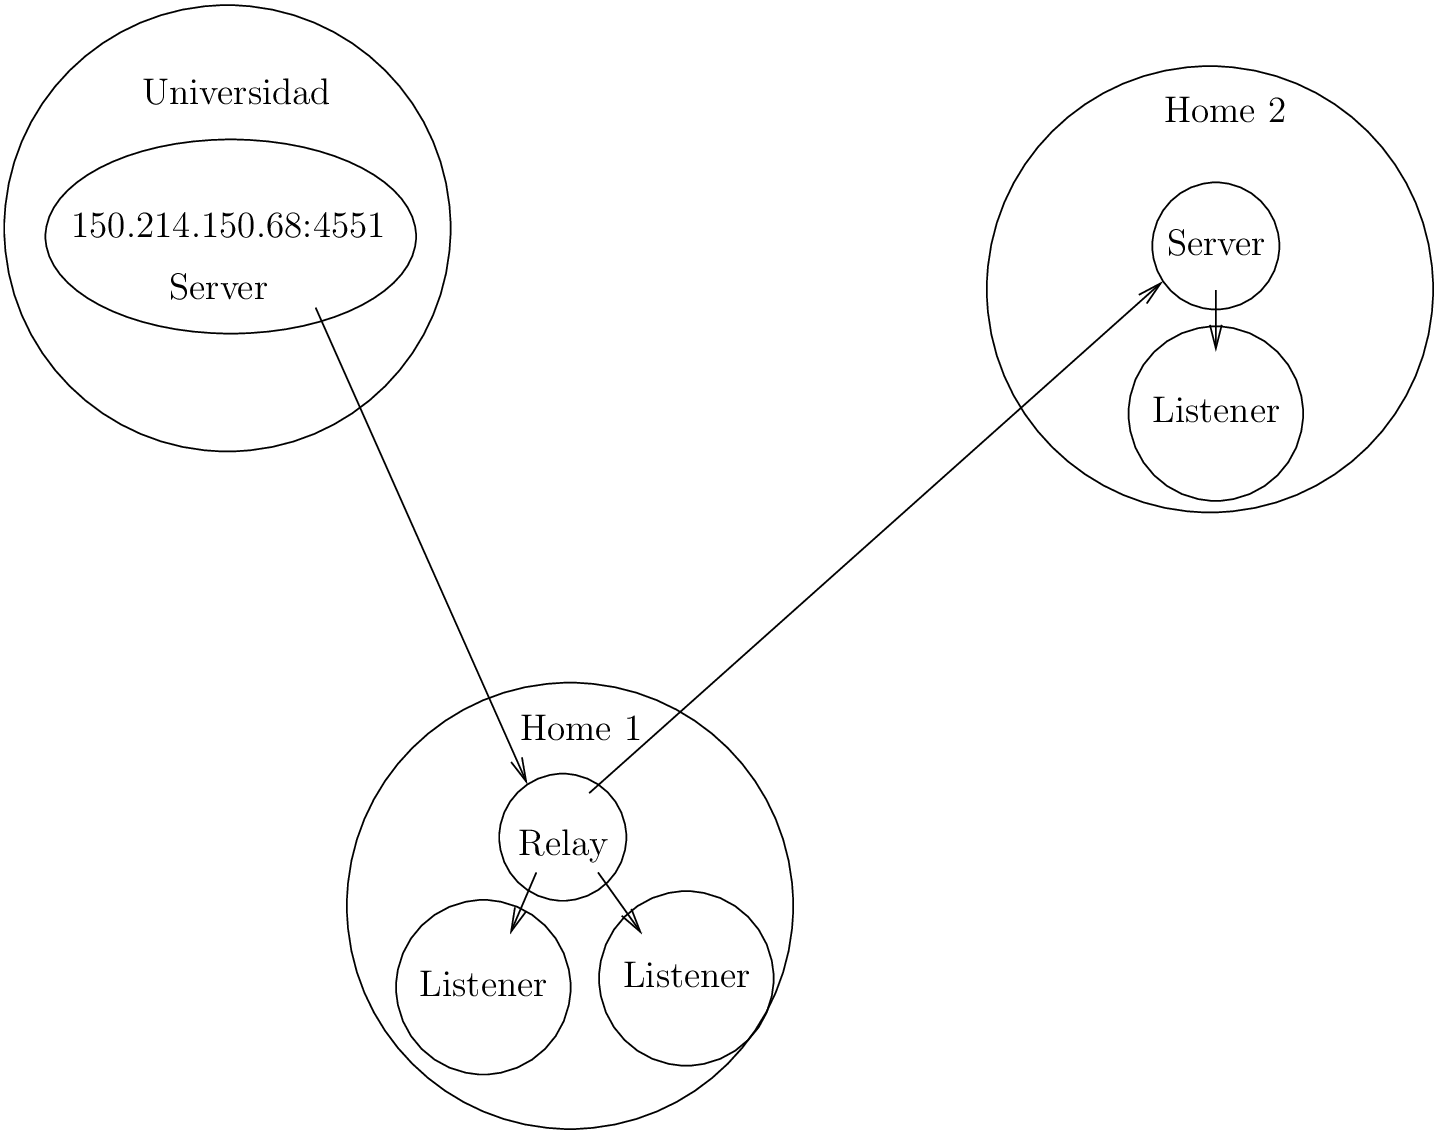
\includegraphics[width=\textwidth]{configuration}
\end{center}

%}}}

\section{Entregables}
%{{{

\begin{enumerate}
\item Una descripci\'on de los experimentos realizados.
\item El contenido del fichero \texttt{/etc/icecast2/icecast.xml}.
\end{enumerate}

%}}}

\section*{Virtual Box + NAT + Port Forwarding}
Hay que definir una regla en el menu: Configuración - Red -
Adaptador 1 - Reenvío de puertos: Ejemplo regla:
\begin{verbatim}
Nombre  | Protocolo | IP anfitrion | Puerto anfitrion | IP invitado | Puerto invitado
Regla 1 |       TCP |  192.168.1.3 |             2222 |   10.0.2.15 | 22
\end{verbatim}

Es importante que especifiquemos la IP del anfitri\'on (y no 127.0.0.1,
por ejemplo) o de lo contrario no podremos conectarnos desde fuera del
host anfitrion hacia el host virtual. Ejemplo de conexi\'on (incluso
desde un host diferente a \texttt{192.168.1.3}):
\begin{verbatim}
ssh -p 2222 192.168.1.3
\end{verbatim}

%}}}

\end{comment}